\documentclass{beamer}
\usefonttheme[onlylarge]{structuresmallcapsserif}
\usefonttheme[onlysmall]{structurebold}
\usetheme{Warsaw}
\setbeamercovered{transparent}
%-----------------------------------------Paquetes y comandos personales-------------------------------%
\usepackage{fancybox,color,tcolorbox}
\usepackage{verbatim}
\usepackage[english,spanish,activeacute]{babel}
%\usepackage[latin1]{inputenc}
\usepackage{inputenc}
\usepackage{latexsym}
\usepackage{amsmath}
\usepackage{graphicx} % Allows including images
\usepackage{booktabs}
\usepackage{amssymb}
\usepackage{multimedia}
\usepackage{pifont,pgfcore}
\usepackage{tcolorbox}
\usepackage{animate}
\usepackage{ucs}
%-----------------------------------------------------Nuevos Ambientes----------------------------------%

\newtheorem*{Theorem*}{Teorema}
\newtheorem*{Definition*}{Definici'on}
\newtheorem*{Example*}{Ejemplo}

%-----------------------------------------------------Nuevos Comandos-----------------------------------%
%-----------------------------------------------------Titulo--------------------------------------------%
\title[Cabrera]{Moogle!}
\author[Dayan]{Dayan Cabrera Corvo}
\date{\today}

\begin{document}
%-----Redefiniendo colores----------%
\definecolor{green}{rgb}{0.1,0.5,0.3}
\definecolor{vio}{rgb}{0.8,0.5,0.2}
\definecolor{g}{rgb}{0.93,0.93,0.93}
\begin{frame}
 \titlepage
  \begin{center}
    \colorbox{black}{\textbf{\begin{large}\textcolor{white}{Un buscador eficiente.}\end{large}}}\\\ \\
    \scriptsize \textbf{\textcolor{blue}{Facultad Matem\'atica Computaci\'on}}\\
    \textbf{\textcolor{blue}{Universidad de La Habana}}
  \end{center}
\end{frame}
%-----------------------------------------------

%-------------------------------------------------
\begin{frame}
	\frametitle{Temas a tratar} 
	\tableofcontents 
\end{frame}
%------------------------------------

%-------------------------------------
\section{Introducci\'on}
\begin{frame}
\begin{minipage}{10cm}
	 Moogle! es una aplicación totalmente original cuyo propósito es buscar inteligentemente un texto en un conjunto de documentos. Es una aplicación web, desarrollada con tecnología .NET Core 6.0, específicamente usando Blazor como framework web para la interfaz gráfica. La aplicación está dividida en dos componentes fundamentales: MoogleServer es un servidor web que renderiza la interfaz gráfica y sirve los resultados. MoogleEngine es una biblioteca de clases donde está implementada la lógica del algoritmo de búsqueda. 
\end{minipage}
\end{frame}

\section{Formulaci\'on matem\'atica}

\begin{frame}
\frametitle{Modelo matemático}
\begin{minipage}{10cm}
	La formulación general del modelo utilizado es TF IDF \\
	\begin{equation}\label{eq:general}
			\begin{cases}
			TF = n/N   \\
			IDF = log(1+D/d)
			\end{cases}
	\end{equation} 
	La variable $''n''$ representa la cantidad de apariciones de una palabra en un documento y $''N''$ representa la cantidad de palabras del documento. En el caso del IDF la variable $''D''$ representa la cantidad de documentos existentes y $''d''$ la cantidad de documentos que contienen la palabra en cuestion. \\
	De esta forma al realizar la multiplicacion del TF y el IDF, obtendriamos la relvancia de esa palabra en esos documentos.
\end{minipage}

\end{frame}	

\begin{frame}
	% \frametitle{Modelo matemático}
	\begin{minipage}{10 cm}
		Una vez calculado el TDIDF de todos los documentos se procede de la siguiente forma:
		\begin{itemize}
			\item Si $TFIDF=0$, el documento no tendria relevancia y no se moestraria.
			equilibrio.
			\item Si $TFIDF > 0$, el documento se compararia con otros y se mostrarian en orden descendente.
		\end{itemize}
	Una ves hecho esto los documentos quedan organizados por orden de relevancia.
	\end{minipage}
\end{frame}

\begin{frame}
	% \frametitle{Modelo matemático}
	\begin{minipage}{10 cm}
La distancia de Levenshtein, distancia de edición o distancia entre palabras es el número mínimo de operaciones requeridas para transformar una cadena de caracteres en otra, se usa ampliamente en teoría de la información y ciencias de la computación. Se entiende por operación, bien una inserción, eliminación o la sustitución de un carácter. Esta distancia recibe ese nombre en honor al científico ruso Vladimir Levenshtein, quien se ocupó de esta distancia en 1965. Es útil en programas que determinan cuán similares son dos cadenas de caracteres, como es el caso de los correctores ortográficos. 
		\begin{itemize}
			\item casa cala(sustitucion 's' por 'l')
			\item cala calla(insercion de 'l' ente 'l' y 'a')
                   \item  calla calle(sustitucion de 'a' por 'e')
		\end{itemize}
	\end{minipage}
\end{frame}

\begin{figure}[h]
    \centering
	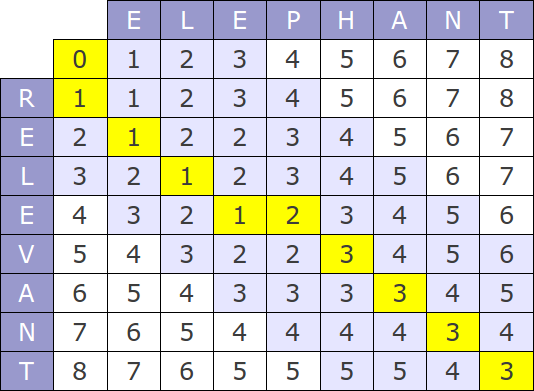
\includegraphics[width=0.68\textwidth]{imagenes/diagrama.png}
    \caption{Ejemplo de distancia de Lvenshtein}
    \label{img:3}
\end{figure}







\begin{frame}
	\frametitle{Funcionalidades del Moogle}
	\begin{minipage}{10 cm}
		Cuando el programa se ejecuta, en primer lugar se extraen los txt de la ruta asignada, estos textos se procesan y luego a partir de ellos se calcula el TD, el IDF y el TF-IDF para cada palabra diferente en el documento. Una vez procesada toda esta informacion ya las busquedas saldrian mas rapido. Ahora, las busquedas a su vez son procesadas y llevadas a un array que se ira multiplicando por la (Matriz) con los TFIDF de cada texto, luego se le aplicarian los cambios con respecto a los simbolos y esto nos daria el escore de cada texto. En caso de que una palabra de la busqueda no se encuentre en el conjunto de textos, Moogle le enviara una sugerencia, eso aplica a su vez para palabras mal escritas. 
Cuenta a su vez con caracteres especiales de busqueda: ('!', '\^{}', '~', '*')
	\end{minipage}
\end{frame}





\begin{frame}
	\frametitle{Caracteres especiales}
	\begin{minipage}{10cm}
	\begin{alertblock}{'!'}
		 Delante de una palabra devuelve txt donde esta palabra no puede aparecer.
	\end{alertblock}
	\begin{alertblock}{'\^{}'}
		Delante de una palabra devuelve txt donde esa palabra tiene que aprecer obligatoriamente.
	\end{alertblock}

      \begin{alertblock}{'*'}
            Delante de una palabra, le da a esta palabra mas relevancia en la busqueda. 
      \end{alertblock} 
	\end{minipage}
\end{frame}




%----------------------------------
\section{Conclusiones}

\begin{frame}
	\frametitle{Conclusiones}
	\begin{minipage}{10cm}
		En resumen Moogle! es un buscador solo de txt basado en un modelo vectorial(TFIDF), se usan ademas otros algoritmos compo la distancia de Levenshtein, creando asi un proyecto considerablemente eficiente.
	\end{minipage}
\end{frame}


\end{document}


